\documentclass{beamer}
\mode<presentation>
\usepackage{amsmath,amssymb,mathtools}
\usepackage{textcomp}
\usepackage{gensymb}
\usepackage{adjustbox}
\usepackage{subcaption}
\usepackage{enumitem}
\usepackage{multicol}
\usepackage{listings}
\usepackage{url}
\usepackage{graphicx} % <-- needed for images
\def\UrlBreaks{\do\/\do-}

\usetheme{Boadilla}
\usecolortheme{lily}
\setbeamertemplate{footline}{
  \leavevmode%
  \hbox{%
  \begin{beamercolorbox}[wd=\paperwidth,ht=2ex,dp=1ex,right]{author in head/foot}%
    \insertframenumber{} / \inserttotalframenumber\hspace*{2ex}
  \end{beamercolorbox}}%
  \vskip0pt%
}
\setbeamertemplate{navigation symbols}{}

\lstset{
  frame=single,
  breaklines=true,
  columns=fullflexible,
  basicstyle=\ttfamily\tiny   % tiny font so code fits
}

\numberwithin{equation}{section}

% ---- your macros ----
\providecommand{\nCr}[2]{\,^{#1}C_{#2}}
\providecommand{\nPr}[2]{\,^{#1}P_{#2}}
\providecommand{\mbf}{\mathbf}
\providecommand{\pr}[1]{\ensuremath{\Pr\left(#1\right)}}
\providecommand{\qfunc}[1]{\ensuremath{Q\left(#1\right)}}
\providecommand{\sbrak}[1]{\ensuremath{{}\left[#1\right]}}
\providecommand{\lsbrak}[1]{\ensuremath{{}\left[#1\right.}}
\providecommand{\rsbrak}[1]{\ensuremath{\left.#1\right]}}
\providecommand{\brak}[1]{\ensuremath{\left(#1\right)}}
\providecommand{\lbrak}[1]{\ensuremath{\left(#1\right.}}
\providecommand{\rbrak}[1]{\ensuremath{\left.#1\right)}}
\providecommand{\cbrak}[1]{\ensuremath{\left\{#1\right\}}}
\providecommand{\lcbrak}[1]{\ensuremath{\left\{#1\right.}}
\providecommand{\rcbrak}[1]{\ensuremath{\left.#1\right\}}}
\theoremstyle{remark}
\newtheorem{rem}{Remark}
\newcommand{\sgn}{\mathop{\mathrm{sgn}}}
\providecommand{\abs}[1]{\left\vert#1\right\vert}
\providecommand{\res}[1]{\Res\displaylimits_{#1}}
\providecommand{\norm}[1]{\lVert#1\rVert}
\providecommand{\mtx}[1]{\mathbf{#1}}
\providecommand{\mean}[1]{E\left[ #1 \right]}
\providecommand{\fourier}{\overset{\mathcal{F}}{ \rightleftharpoons}}
\providecommand{\system}{\overset{\mathcal{H}}{ \longleftrightarrow}}
\providecommand{\dec}[2]{\ensuremath{\overset{#1}{\underset{#2}{\gtrless}}}}
\newcommand{\myvec}[1]{\ensuremath{\begin{pmatrix}#1\end{pmatrix}}}
\let\vec\mathbf

\title{MatGeo Presentation - Problem 9.8.1}
\author{EE25BTECH11064 - Yojit Manral}
\date{}

\begin{document}

\frame{\titlepage}
\begin{frame}{Question}
The line $x + 3y = 0$ is the diameter of the circle $x^2 + y^2 - 6x + 2y = 0$.
\end{frame}

\begin{frame}{Solution}
$\rightarrow$ The given circle can be expressed as
\begin{align}
    \vec{x}^T\vec{V}\vec{x} + 2\vec{u}^T\vec{x} + f = 0 \\
    \vec{V} = \myvec{1&0\\0&1}\text{, } \vec{u} = \myvec{-3\\1}\text{, } f = 0
\end{align}
$\rightarrow$ Also, the center of the circle is
\begin{align}
    \vec{c} &= -\vec{V}^{-1}\vec{u}\text{; } |\vec{V}| \neq 0 \\
    \vec{c} &= \myvec{3\\-1}
\end{align}
$\rightarrow$ The given line can be expressed as
\begin{align}
    \vec{x} = \vec{h} + \kappa\vec{m}\text{; } \kappa \in R\\
    \vec{h} = \myvec{0\\0}\text{, } \vec{m} = \myvec{3\\-1}
\end{align}
$\rightarrow$ If the line is a diameter of the circle, the center of the circle must lie on the line
\end{frame}

\begin{frame}{Solution}
\begin{align}
    \vec{c} &= \vec{h} + \lambda \vec{m} \hspace{0.2cm} \exists \hspace{0.1cm} \lambda \in R \\
    \myvec{3\\-1} &= \myvec{0\\0} + \lambda \myvec{3\\-1} \implies \lambda = 1 \in R
\end{align}
$\implies$ $\vec{c}$ lies on the line $\implies$ The line is a diameter of the circle
\begin{figure}[h!]
   \centering
   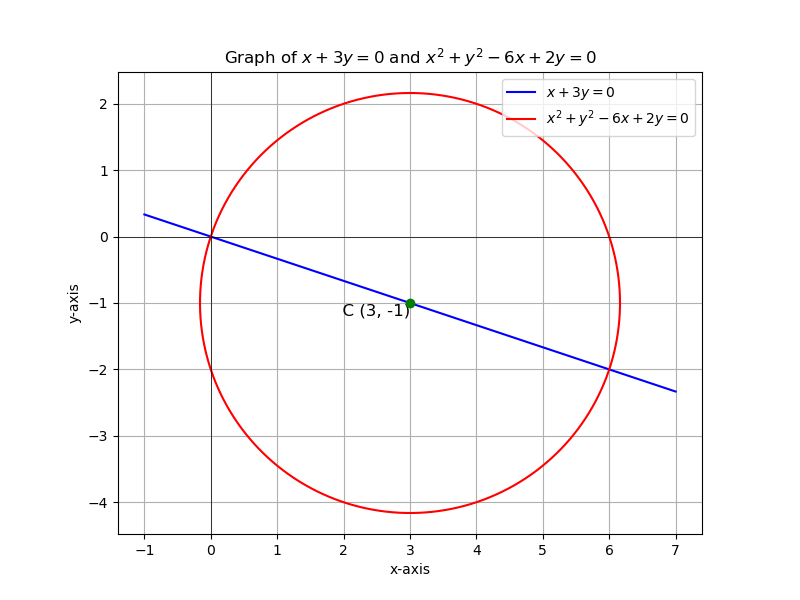
\includegraphics[width=0.54\linewidth]{figs/01.png}
   \caption{Plot of given line and circle}
   \label{Plot_1}
\end{figure}
\end{frame}
 % --------- CODE APPENDIX ---------
\section*{Appendix: Code}
% Python plotting
\begin{frame}[fragile]{File: plot.py}
\begin{lstlisting}[language=Python]
import numpy as np
import matplotlib.pyplot as plt

# Define the equation of the line
def line(x):
    return -x / 3
# Create x values for the line
x_vals = np.linspace(-1, 7, 400)
y_vals = line(x_vals)

# Circle equation
theta = np.linspace(0, 2 * np.pi, 400)
x_circle = 3 + np.sqrt(10) * np.cos(theta)
y_circle = -1 + np.sqrt(10) * np.sin(theta)

# Plot the line and the circle and the center
plt.figure(figsize=(8, 8))
plt.plot(x_vals, y_vals, label=r'$x + 3y = 0$', color='blue')  # Line equation
plt.plot(x_circle, y_circle, label=r'$x^2 + y^2 - 6x + 2y = 0$', color='red')  # Circle equation
plt.scatter(3, -1, color='green', zorder=5)  # Green dot for the center
plt.text(3, -1, '  C (3, -1)', fontsize=12, verticalalignment='top', horizontalalignment='right')

# Setting up the plot
plt.axhline(0, color='black',linewidth=0.5)
plt.axvline(0, color='black',linewidth=0.5)
plt.gca().set_aspect('equal', adjustable='box')  # To ensure the circle looks like a circle
plt.legend()
plt.title("Graph of $x + 3y = 0$ and $x^2 + y^2 - 6x + 2y = 0$")
plt.xlabel("x-axis")
plt.ylabel("y-axis")
plt.grid(True)
plt.show()
\end{lstlisting}
\end{frame}

\end{document}
